\documentclass[]{beamer}

\setbeamertemplate{caption}[numbered]
\setbeamertemplate{caption label separator}{:}
\setbeamercolor{caption name}{fg=normal text.fg}
\usepackage{amssymb,amsmath}
\usepackage{ifxetex,ifluatex}
\usepackage{fixltx2e} % provides \textsubscript
\usepackage{lmodern}
\ifxetex
  \usepackage{fontspec,xltxtra,xunicode}
  \defaultfontfeatures{Mapping=tex-text,Scale=MatchLowercase}
  \newcommand{\euro}{€}
\else
  \ifluatex
    \usepackage{fontspec}
    \defaultfontfeatures{Mapping=tex-text,Scale=MatchLowercase}
    \newcommand{\euro}{€}
  \else
    \usepackage[T1]{fontenc}
    \usepackage[utf8]{inputenc}
      \fi
\fi
% use upquote if available, for straight quotes in verbatim environments
\IfFileExists{upquote.sty}{\usepackage{upquote}}{}
% use microtype if available
\IfFileExists{microtype.sty}{\usepackage{microtype}}{}
\usepackage{bm}

% Comment these out if you don't want a slide with just the
% part/section/subsection/subsubsection title:
% \AtBeginPart{
%   \let\insertpartnumber\relax
%   \let\partname\relax
%   \frame{\partpage}
% }
% \AtBeginSection{
%   \let\insertsectionnumber\relax
%   \let\sectionname\relax
%   \frame{\sectionpage}
% }
% \AtBeginSubsection{
%   \let\insertsubsectionnumber\relax
%   \let\subsectionname\relax
%   \frame{\subsectionpage}
% }
\usepackage{tikz}
\usetikzlibrary{decorations.pathreplacing,calc}
\newcommand{\tikzmark}[1]{\tikz[overlay,remember picture] \node (#1) {};}

\setbeamersize{text margin left=2em,text margin right=2em}
\setlength{\parindent}{0pt}
\setlength{\parskip}{6pt plus 2pt minus 1pt}
\setlength{\emergencystretch}{3em}  % prevent overfull lines
\setcounter{secnumdepth}{0}
\providecommand{\tightlist}{%
  \setlength{\itemsep}{0pt}\setlength{\parskip}{0pt}}

\DeclareMathOperator*{\argmin}{arg\,min}

\newcommand{\twopartdef}[4]
{
  \left\{
    \begin{array}{ll}
      #1 & \mbox{if } #2 \\
      #3 & \mbox{if } #4
    \end{array}
  \right.
}

\newcommand{\twopartdefo}[3]
{
  \left\{
    \begin{array}{ll}
      #1 & \mbox{if } #2 \\
      #3 & \mbox{otherwise}
    \end{array}
  \right.
}

%gets rid of bottom navigation bars
\setbeamertemplate{footline}[frame number]{}

%gets rid of navigation symbols
\setbeamertemplate{navigation symbols}{}
\usebackgroundtemplate{
  \tikz[overlay,remember picture] 
  \node[opacity=0.4, at=(current page.north east),anchor=north east] {
    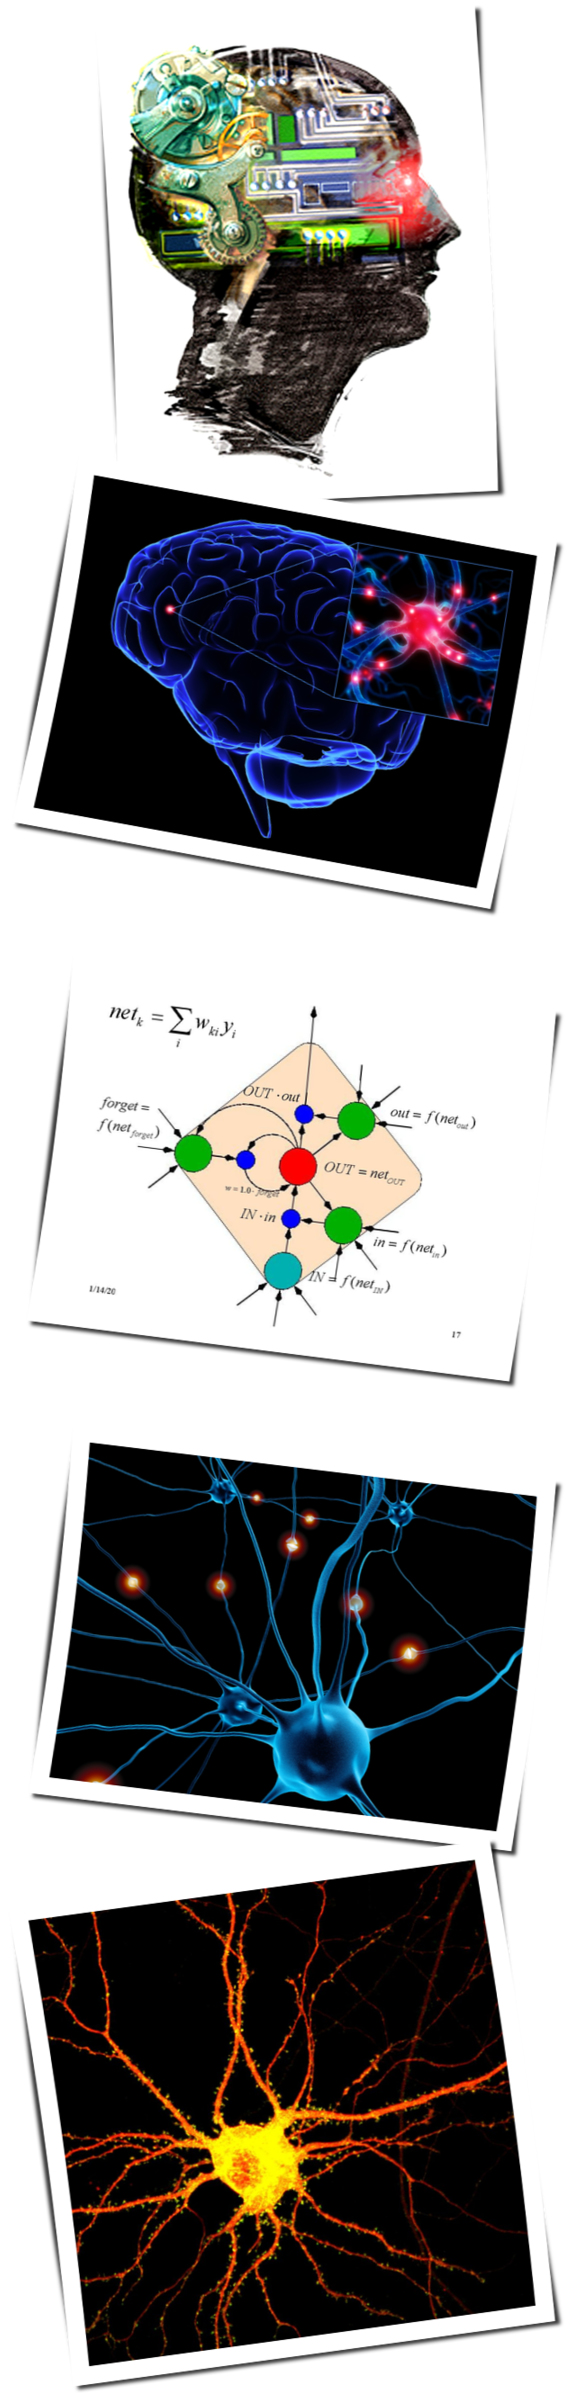
\includegraphics[width=0.17\paperwidth]{figures/nn.jpg}};
}

\DeclareMathOperator*{\argmax}{arg\,max}

\title{A (gentle) introduction to ~}
\date{}

\begin{document}
\frame{\titlepage}

\begin{frame}
\tableofcontents[hideallsubsections]
\end{frame}

\begin{frame}

Reinforcement Learning \% Spyros Samothrakis \% August 28, 2014

\end{frame}

\section{Introduction \& Motivation}\label{introduction-motivation}

\usebackgroundtemplate{

}

\begin{frame}{What is Reinforcement Learning?}

\begin{itemize}
\tightlist
\item
  \emph{Reinforcement learning is the study of how animals and
  artificial systems can learn to optimize their behavior in the face of
  rewards and punishments} -- Peter Dyan, Encyclopedia of Cognitive
  Science
\item
  \textbf{Not} supervised learning - the animal/agent is not provided
  with examples of optimal behaviour, it has to be discovered!
\item
  \textbf{Not} unsupervised learning either - we have more guidance than
  just observations
\end{itemize}

\end{frame}

\begin{frame}{Links to other fields}

\begin{itemize}
\tightlist
\item
  It subsumes most artificial intelligence problems
\item
  Forms the basis of most modern intelligent agent frameworks
\item
  Ideas drawn from a wide range of contexts, including psychology (e.g.,
  Skinner's ``Operant Conditioning''), philosophy, neuroscience,
  operations research
\end{itemize}

\end{frame}

\begin{frame}{Examples of Reinforcement Learning closer to CS}

\begin{itemize}
\tightlist
\item
  Play backgammon/chess/go/poker/any game (at human or superhuman level)
\item
  Helicopter control
\item
  Learn how to walk/crawl/swim/cycle
\item
  Elevator scheduling
\item
  Optimising a petroleum refinery
\item
  Optimal drug dosage
\end{itemize}

\end{frame}

\section{Markov Decision Process
(MDPs)}\label{markov-decision-process-mdps}

\begin{frame}{The Markov Decision Process}

\begin{itemize}
\tightlist
\item
  The primary abstraction we are going to work with is the Markov
  Decision Process (MDP).
\item
  MDPs capture the dynamics of a mini-world/universe/environment
\item
  An MDP is defined as a tuple \(<S,A,T,R,\gamma>\) where:

  \begin{itemize}
  \tightlist
  \item
    \(S\), \(s \in S\) is a set of states
  \item
    \(A\), \(a \in A\) is a set of actions
  \item
    \(R:S \times A\), \(R(s,a)\) is a function that maps state-actions
    to rewards
  \item
    \(T:S\times S\times A\), with \(T(s'| s, a)\) being the probability
    of an agent landing from state \(s\) to state \(s'\) after taking
    \(a\)
  \item
    \(\gamma\) is a discount factor - the impact of time on rewards
  \end{itemize}
\end{itemize}

\end{frame}

\begin{frame}{The Markov Property and States}

\begin{itemize}
\tightlist
\item
  States represent sufficient statistics.
\item
  Markov Property ensures that we only care about the present in order
  to act - we can safely ignore past states
\item
  Think Tetris - all information are can be captured by a single
  screen-shot
\end{itemize}

\begin{columns}[T] % align columns
\begin{column}{.48\textwidth}
\color{red}\rule{\linewidth}{4pt}
First DOS Version

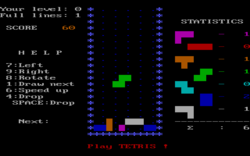
\includegraphics[scale=0.60]{figures/250px-Tetris_DOS_1986.png}
\end{column}%
\hfill%
\begin{column}{.48\textwidth}
\color{blue}\rule{\linewidth}{4pt}
Original Tetris

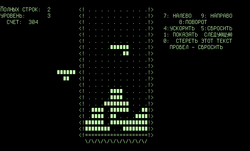
\includegraphics[scale=0.60]{figures/250px-Tetris-VeryFirstVersion.png}
\end{column}%
\end{columns}

\end{frame}

\begin{frame}{Agents, Actions and Transitions}

\begin{itemize}
\tightlist
\item
  An agent is an entity capable of actions
\item
  An MDP can capture any environment that is inhabited either by

  \begin{itemize}
  \tightlist
  \item
    Exactly one agent
  \item
    Multiple agents, but only one is adaptive
  \end{itemize}
\item
  Notice how actions are part of the MDP - notice also how the MDP is a
  ``world model''
\item
  The agent is just a ``brain in a vat''
\item
  The agent perceives states/rewards and outputs actions
\item
  Transitions specify the effects of actions in the world (e.g., in
  Tetris, you push a button, the block spins)
\end{itemize}

\end{frame}

\begin{frame}{Rewards and the Discount Factor}

\begin{itemize}
\tightlist
\item
  Rewards describe state preferences
\item
  Agent is happier in some states of the MDP (e.g., in Tetris when the
  block level is low, a fish in water, pacman with a high score)
\item
  Punishment is just low/negative reward (e.g., being eaten in pacman)
\item
  \(\gamma\), the discount factor,

  \begin{itemize}
  \tightlist
  \item
    Describes the impact of time on rewards
  \item
    ``I want it now'', the lower \(\gamma\) is the less important future
    rewards are
  \end{itemize}
\item
  There are no ``springs/wells of rewards'' in the real world

  \begin{itemize}
  \tightlist
  \item
    What is ``human nature''?
  \end{itemize}
\end{itemize}

\end{frame}

\begin{frame}{Examples of Reward Schemes}

\begin{itemize}
\tightlist
\item
  Scoring in most video games
\item
  The distance a robot walked for a bipedal robot
\item
  The amount of food an animal eats
\item
  Money in modern societies
\item
  Army Medals (``Gamification'')
\item
  Vehicle routing

  \begin{itemize}
  \tightlist
  \item
    (-Fuel spend on a flight)
  \item
    (+ Distance Covered)
  \end{itemize}
\item
  Cold/Hot
\end{itemize}

\end{frame}

\begin{frame}{Long Term Thinking}

\begin{itemize}
\tightlist
\item
  It might be better to delay satisfaction
\item
  Immediate reward is not always the maximum reward
\item
  In some settings there are no immediate rewards at all (e.g., most
  solitaire games)
\item
  MDPs and RL capture this
\item
  ``Not going out tonight, study''
\item
  Long term investment
\end{itemize}

\end{frame}

\begin{frame}{Policy}

\begin{itemize}
\tightlist
\item
  The MDP (the world) is populated by an agent (an actor)
\item
  You can take actions (e.g., move around, move blocks)
\item
  The type of actions you take under a state is called the \emph{policy}
\item
  \(\pi: S \times A\), \(\pi(s,a) = P(a|s)\), a probabilistic mapping
  between states and actions
\item
  Finding an optimal policy is \emph{mostly} what the RL problem is all
  about
\end{itemize}

\end{frame}

\begin{frame}{The Full Loop}

\begin{itemize}
\tightlist
\item
  See how the universe described by the MDP defines actions, not just
  states and transitions
\item
  An agent needs to act upon what it perceives
\item
  Notice the lack of body - ``brain in a vat''. Body is assumed to be
  part of the world.
\item
  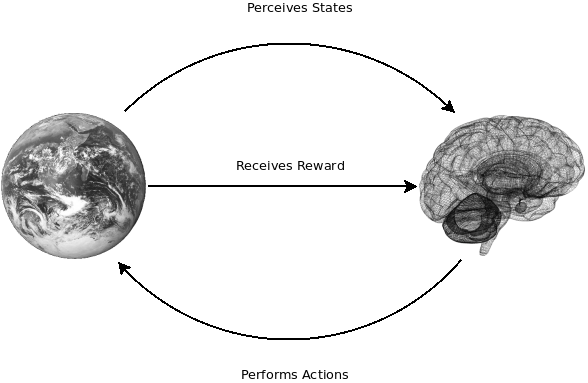
\includegraphics[scale=0.33]{figures/RL.png}
\end{itemize}

\end{frame}

\begin{frame}{Example MDP - EagleWorld}

\center
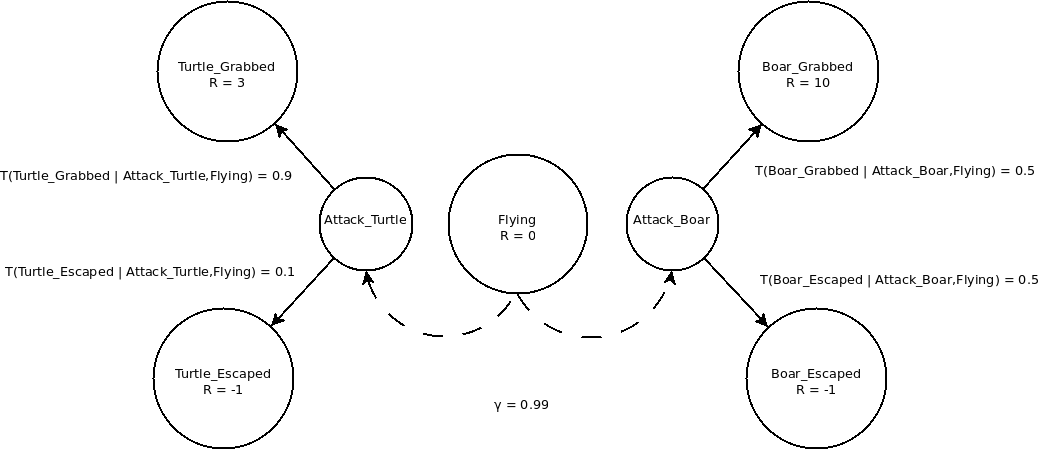
\includegraphics[scale=0.33]{figures/MDPExample-simple2.png}

\end{frame}

\begin{frame}{Agent Goals}

\begin{itemize}
\item
  The agent's goal is to maximise its long term reward
  \(\mathbb{E}_{\pi}\left[\sum\limits_{t=0}^\infty{\gamma^tR \left( s^{t},a^t \right)}\right]\)
\item
  Risk Neutral Agent - think of the EagleWorld example
\item
  Rewards can be anything, but most organisms receive rewards only in a
  very limited amount of states (e.g., fish in water)
\item
  What if your reward signal is only money?

  \begin{itemize}
  \tightlist
  \item
    Sociopathic, egotistic, greed-is-good Gordon Gekko (\emph{Wall
    Street}, 1987)
  \item
    No concept of ``externalities'' - agents might wreak havoc for
    marginal reward gains
  \item
    Same applies to all ``compulsive agents'' - think Chess
  \end{itemize}
\end{itemize}

\end{frame}

\begin{frame}{Searching for a good Policy}

\begin{itemize}
\tightlist
\item
  One can possibly search through all combinations of policies until she
  finds the best
\item
  Slow, does not work in larger MDPs
\item
  Exploration/Exploitation dilemma

  \begin{itemize}
  \tightlist
  \item
    How much time/effort should be spend exploring for solutions?
  \item
    How much time should be spend exploiting good solutions?
  \end{itemize}
\end{itemize}

\end{frame}

\section{Model Based Reinforcement
Learning}\label{model-based-reinforcement-learning}

\begin{frame}{Model Based Reinforcement Learning}

\begin{itemize}
\tightlist
\item
  \ldots{}also known as planning in certain contexts
\item
  Who was doing the thinking in the previous example (You? The eagle?)
\item
  An agent has access to model, i.e., has a copy of the MDP (the outside
  world) in its mind
\item
  Using that copy, it tries to ``think'' what is the best route of
  action
\item
  It then executes this policy on the real world MDP
\item
  You can't really copy the world inside your head, but you can copy the
  dynamics
\item
  ``This and that will happen if I push the chair''
\item
  Thinking, introspection\ldots{}
\end{itemize}

\end{frame}

\begin{frame}{Bellman Expectation Equations / Bellman Backups}

\begin{itemize}
\tightlist
\item
  The two most important equations related to MDP
\item
  Recursive definitions
\item
  \(V^\pi (s) = \sum\limits_{a \in A}\pi(s,a) \left( R(s,a) + \gamma\sum\limits_{s' \in S}T(s'|s,a) V^\pi(s') \right)\)
\item
  \(Q^\pi (s,a) = R(s,a) + \gamma\sum\limits_{s' \in S} T(s'|s,a) \sum\limits_{a' \in A} \pi(s',a')Q^\pi(s',a')\)
\item
  \textbf{Called V-Value(s) (\emph{state-value function}) and Q-Value(s)
  (\emph{state-action value function}) respectively}
\item
  Both calculate the expected rewards under a certain policy
\end{itemize}

\end{frame}

\begin{frame}{Link between \(V^\pi\) and \(Q^\pi\)}

\begin{itemize}
\tightlist
\item
  \(V\) and \(Q\) are interrelated
\item
  \(V^\pi(s) = \sum\limits_{a \in A} \pi(s,a) Q^\pi(s,a)\)
\item
  \(Q^\pi(s,a) = R(s,a) + \sum\limits_{s' \in S} T(s'|s,a) V^\pi(s')\)
\end{itemize}

\end{frame}

\begin{frame}{Example MDP - EagleWorld - Random Policy}

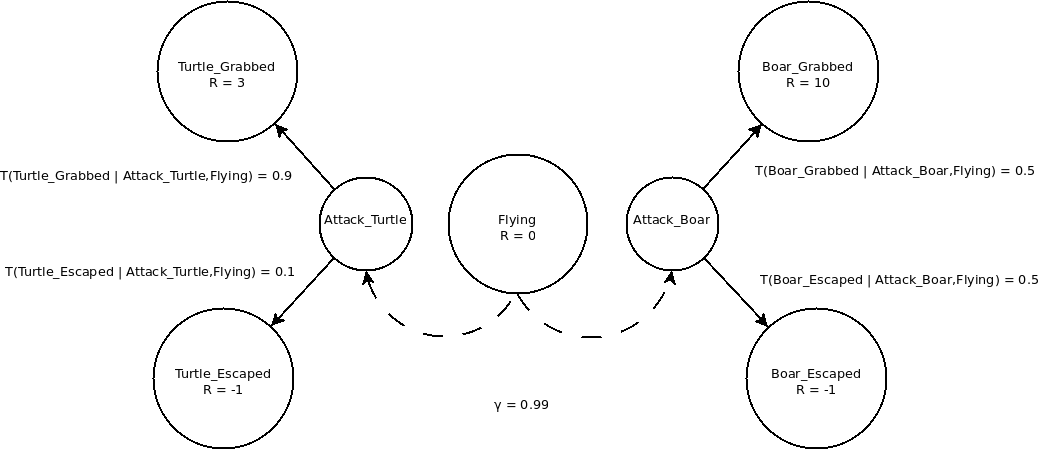
\includegraphics[scale=0.33]{figures/MDPExample-simple2.png}

\small
\center
\textcolor{red}{
$\pi(Flying, Attack\_Boar) = 0.5, \pi(Flying,Attack\_Turtle) = 0.5$
$Q(Flying, Attack\_Boar)   = 0.99 * (10 * 0.5 + 0.5*-1) = 4.455$
$Q(Flying, Attack\_Turtle) = 0.99 * (0.9 * 3 + 0.1*-1) = 2.574$
$V^\pi(Flying) = 0.5, Q^\pi(Flying, Attack\_Turtle) +0.5, Q(Flying, Attack\_Boar) = 3.5145$
}

\end{frame}

\begin{frame}{Optimal Policy and the Bellman Optimality Equation}

\begin{itemize}
\tightlist
\item
  An optimal policy can be defined in terms of Q-values
\item
  It is the policy that maximises \(Q\) values
\item
  \(V^* (s) = \max\limits_{a \in A}R(s,a) + \gamma\sum\limits_{s' \in S}T(s'|s,a) V^*(s')\)
\item
  \(Q^* (s,a) = R(s,a) + \gamma\sum\limits_{s' \in S} T(s'|s,a) \max\limits_{a' \in A} Q^*(s',a')\)
\item
  \(\pi^*(s,a) = \twopartdefo{ 1 } {a = \argmax\limits_{a \in A} Q^*(s,a)} {0}\)
\end{itemize}

\end{frame}

\begin{frame}{Link between \(V^*\) and \(Q^*\)}

\begin{itemize}
\tightlist
\item
  Again, they are interrelated
\item
  \(V(s)^* = \max\limits_{a \in A} Q^*(s,a)\)
\item
  \(Q^*(s,a) = R(s,a) + \gamma\sum\limits_{s' \in S} T(s'|s,a) V^*(s')\)
\end{itemize}

\end{frame}

\begin{frame}{Example MDP - EagleWorld - Optimal Policy}

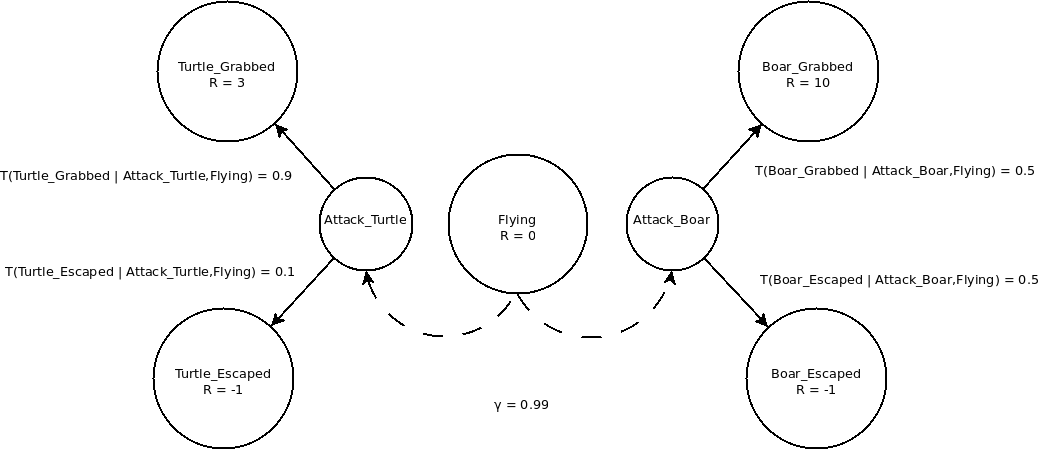
\includegraphics[scale=0.33]{figures/MDPExample-simple2.png}

\small
\center
\textcolor{red}{
$Q(Flying, Attack\_Boar)   = 0.99 * (10 * 0.5 + 0.5*-1) = 4.455$
$Q(Flying, Attack\_Turtle) = 0.99 * (0.9 * 3 + 0.1*-1) = 2.574$
$\pi^*(Flying, Attack\_Boar) = 1$, $\pi^*(Flying,Attack\_Turtle) = 0$
$V^*(Flying) =  Q(Flying,Attack\_Boar) = 4.455 $
}

\end{frame}

\begin{frame}{Agents Revisited}

\begin{itemize}
\tightlist
\item
  An Agent can be composed of a number of things
\item
  A policy
\item
  A Q-Value/and or V-Value Function
\item
  A Model of the environment (the MDP)
\item
  Inference/Learning Mechanisms
\item
  \ldots{}
\item
  An agent has to be able to \emph{create a policy} either on the fly or
  using Q-Values
\item
  The Model/Q/V-Values serve as intermediate points towards constructing
  a policy
\end{itemize}

\end{frame}

\section{Model Free Reinforcement
Learning}\label{model-free-reinforcement-learning}

\begin{frame}{Simplifying assumptions}

\begin{itemize}
\tightlist
\item
  Assume deterministic transitions
\item
  Thus, taking an action on a state will lead only to ONE other possible
  state for some action \(a_c\)

  \begin{itemize}
  \tightlist
  \item
    \(T(s'|s,a_i) = \twopartdefo{ 1 } {a_i = a_c} {0}\)
  \item
    \(V^*(s) = \max\limits_{a \in A} \left[ R(s,a) + \gamma V^*(s') \right]\)
  \item
    \(Q(s,a) = R(s,a) + \gamma \max\limits_{a' \in A} {{Q}(s',a')}\)
  \end{itemize}
\item
  It is easier now to solve for problems that have loops in them
\item
  We can also attempt to learn Q-Values without a model!
\item
  All we need in order to find the optimal policy is \(Q(s,a)\)
\end{itemize}

\end{frame}

\begin{frame}{Deterministic Q-Learning (1)}

\begin{itemize}
\tightlist
\item
  The policy is deterministic from start to finish
\item
  We will use \(\pi(s) = \argmax\limits_{a \in A} Q(s,a)\) to denote the
  optimal policy
\item
  The algorithm now is:

  \begin{itemize}
  \tightlist
  \item
    Initialise all \(Q(s,a)\) to low values
  \item
    Repeat:

    \begin{itemize}
    \tightlist
    \item
      Select an action \(a\) using an exploration policy
    \item
      \(Q(s,a) \gets R(s,a) + \gamma \max\limits_{a' \in A} {{Q}(s',a')}\)
    \item
      \(s \gets s'\)
    \end{itemize}
  \item
    Also known as ``Dynamic Programming'', ``Value Iteration''
  \end{itemize}
\end{itemize}

\end{frame}

\begin{frame}{An Example (1)}

\center
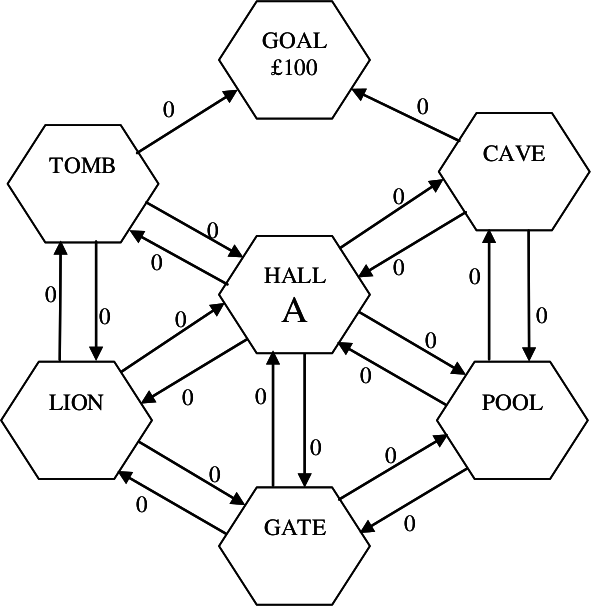
\includegraphics[scale=0.30]{figures/example1.png}

\(R(HALL, To-CAVE) = 0\)

\({Q}(CAVE,a) = 0\) for all actions a

\end{frame}

\begin{frame}{An Example (2)}

Next suppose the agent, now in state CAVE , selects action \(To-GOAL\)

\(R(CAVE, To-GOAL) = 100\), \({Q}(GOAL,a) = 0\) for all actions (there
are no actions)

Hence \({Q}(CAVE, To-GOAL) = 100 + \gamma * 0 = 100\)

\center
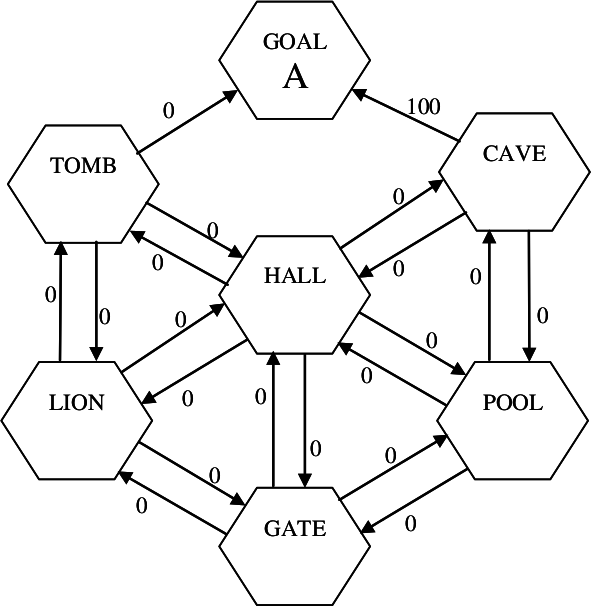
\includegraphics[scale=0.20]{figures/example2.png}

\end{frame}

\begin{frame}{An Example (3)}

Let's start at hall again and select the same action To-CAVE

\(R(HALL, To-CAVE) = 0\), \({Q}(CAVE, GOAL) = 100\)

\({Q}(CAVE,a) = 0\) for all other actions a

Hence \(\max\limits_{a \in A} {Q}(CAVE,a) = 100\), if \(\gamma = 0.8\),
\({Q}(HALL, To-CAVE) = 0 + \gamma * 100 = 80\)

\center
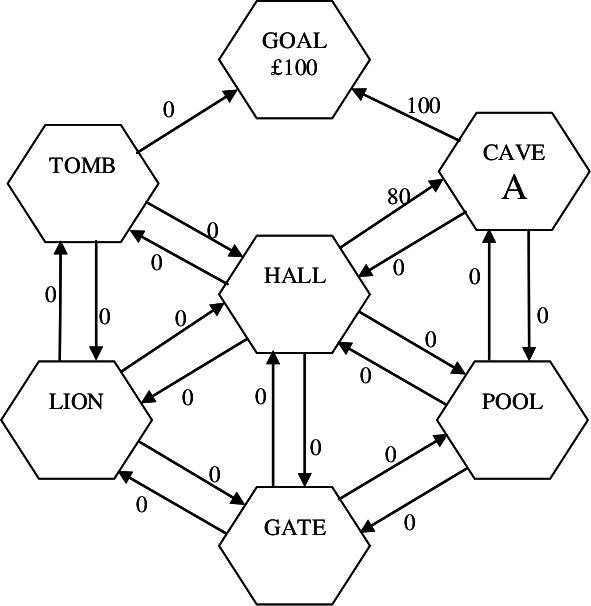
\includegraphics[scale=0.20]{figures/example3.png}

\end{frame}

\begin{frame}{Exploration / Exploitation}

\begin{itemize}
\tightlist
\item
  How do we best explore?
\item
  Choose actions at random - but this can be very slow
\item
  \(\epsilon-greedy\) is the most common method
\item
  Act \(\epsilon\)-greedily

  \begin{itemize}
  \tightlist
  \item
    \(\pi^\epsilon(s,a) = \twopartdefo{ 1-\epsilon + \epsilon/|A| }{ a = \argmax\limits_{a \in A} Q(s,a)}{\epsilon/|A|}\)
  \item
    \(\epsilon\)-greedy means acting greedily with probability
    \(1-\epsilon\), random otherwise
  \end{itemize}
\item
  When you are done, act greedily
  \(\pi(s) = \argmax\limits_{a \in A} Q(s,a)\)
\end{itemize}

\end{frame}

\begin{frame}{Algorithms for non-deterministic settings (1)}

\begin{itemize}
\tightlist
\item
  What can we do if the MDP is not deterministic?
\item
  If we know the model, full blown value iteration
\item
  Otherwise

  \begin{itemize}
  \tightlist
  \item
    Q-learning,
    \(Qs,a) \gets Q(s,a) + \eta\left[R(s,a) + \gamma \max\limits_{a' \in A}Q(s',a') - Q(s,a) \right]\)
  \item
    SARSA(0),
    \(Q(s,a) \gets Q(s,a) + \eta\left[R(s,a) + \gamma Q(s',a') - Q(s,a) \right]\)
  \item
    SARSA(1)/MC,
    \(Q(s,a) \gets Q(s,a) + \eta\left[\mathrm{v_\tau} - Q(s,a)\right]\)
    \(\mathrm{v_\tau} \gets R(s,a)+\gamma R(s',a')+...\gamma^2 R(s'',a'') + \gamma^{\tau-1}R(s^\tau, a^\tau)\)
  \end{itemize}
\item
  \(\eta\) is a small learning rate, e.g., \(\eta = 0.001\)
\end{itemize}

\end{frame}

\begin{frame}{Function Approximation}

\begin{itemize}
\tightlist
\item
  There is usually some link between states
\item
  We can train function approximators incrementally to model \(Q(s,a)\)
\item
  Examples include Linear Function approximators, Neural Networks,
  n-tuple networks
\item
  Not easy to do, few convergance guarrantees

  \begin{itemize}
  \tightlist
  \item
    But with some effort, this works pretty well
  \end{itemize}
\end{itemize}

\end{frame}

\begin{frame}{Relationship to the rest of Machine Learning}

\begin{itemize}
\tightlist
\item
  How can one learn a model of the world?

  \begin{itemize}
  \tightlist
  \item
    Possibly by breaking it down into smaller, abstract chunks

    \begin{itemize}
    \tightlist
    \item
      Unsupervised Learning
    \end{itemize}
  \item
    \ldots{} and learning what effects ones actions have the environment

    \begin{itemize}
    \tightlist
    \item
      Supervised Learning
    \end{itemize}
  \end{itemize}
\item
  RL weaves all fields of Machine Learning (and possibly Artificial
  Intelligence) into one coherent whole
\item
  The purpose of all learning is action!

  \begin{itemize}
  \tightlist
  \item
    You need to be able to recognise faces so you can create state
  \item
    \ldots{} and act on it
  \end{itemize}
\end{itemize}

\end{frame}

\begin{frame}{Conclusion}

\begin{itemize}
\tightlist
\item
  RL is a massive topic
\item
  We have shown the tip of iceberg
\item
  Rabbit hole goes \emph{deep} - both on the application level and the
  theory level
\item
  Essex CS Department has a PhD programme associated with RL

  \begin{itemize}
  \tightlist
  \item
    IGGI Centre
  \item
    Four year long PhD programme
  \item
    Chance to use RL in Computer Games
  \end{itemize}
\end{itemize}

\end{frame}

\begin{frame}{References (1)}

\begin{itemize}
\tightlist
\item
  \textbf{Tom Mitchell, Chapter 13}
\item
  David Silver's UCL Course:
  http://www0.cs.ucl.ac.uk/staff/D.Silver/web/Teaching.html

  \begin{itemize}
  \tightlist
  \item
    Some ideas in these lecture notes taken from there
  \item
    Probably the best set of notes there is on the subject
  \item
    Lectures 1,2,3,4
  \end{itemize}
\item
  Reinforcement Learning, by Richard S. Sutton and Andrew G. Barto

  \begin{itemize}
  \tightlist
  \item
    Classic book
  \item
    Excellent treatment of most subjects
  \item
    Up to Chapter 5
  \end{itemize}
\end{itemize}

\end{frame}

\begin{frame}{References (2)}

\begin{itemize}
\tightlist
\item
  Artificial Intelligence: A Modern Approach by Stuart J. Russell and
  Peter Norvig

  \begin{itemize}
  \tightlist
  \item
    The Introductory A.I. Textbook
  \item
    Chapters 16 and 21
  \end{itemize}
\item
  Algorithms for Reinfocement Learning by Csaba Szepesvari

  \begin{itemize}
  \tightlist
  \item
    Very ``Mathematical'', but a good resource that provides a very
    unified view of the field
  \end{itemize}
\item
  Reinforcement Learning: State-Of-The-Art by Marco Wiering (Editor),
  Martijn Van Otterlo (Editor)

  \begin{itemize}
  \tightlist
  \item
    Edited Volume
  \item
    Chapter 1
  \end{itemize}
\end{itemize}

\end{frame}

\end{document}
